\documentclass[border=4pt]{standalone}
\usepackage{amsmath,amssymb,tikz}
\usetikzlibrary{arrows.meta,calc}
\definecolor{figB}{RGB}{31,90,166}\definecolor{figR}{RGB}{176,48,48}\definecolor{figG}{RGB}{46,125,50}\definecolor{figO}{RGB}{214,120,20}
\begin{document}
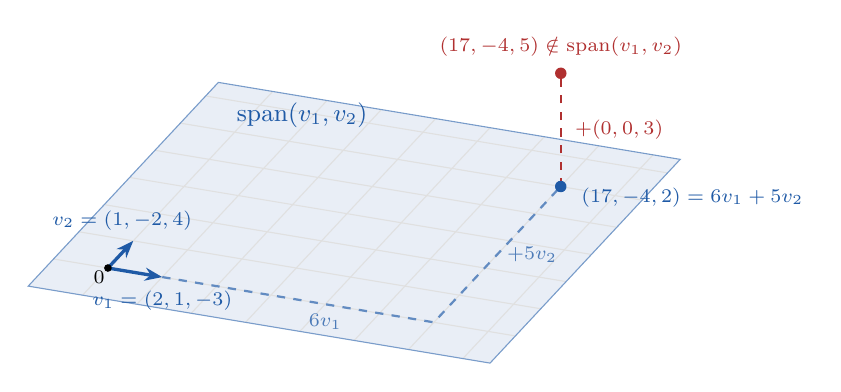
\begin{tikzpicture}[scale=1.15,>={Stealth[length=2.2mm]},x={(0.6cm,-0.1cm)},y={(0.28cm,0.3cm)}]
% plane span(v1,v2) drawn in (s,t)-coordinates s v1 + t v2
\fill[figB!10] (-1,-1)--(7.5,-1)--(7.5,6.5)--(-1,6.5)--cycle;
\foreach \s in {0,...,7} \draw[black!12,thin] (\s,-1)--(\s,6.5);
\foreach \t in {0,...,6} \draw[black!12,thin] (-1,\t)--(7.5,\t);
\draw[figB!60] (-1,-1)--(7.5,-1)--(7.5,6.5)--(-1,6.5)--cycle;
\node[figB,font=\small,anchor=north west] at (-0.7,6.2) {$\operatorname{span}(v_1,v_2)$};
\draw[figB!70,dashed,thick] (1,0)--(6,0)--(6,5);
\draw[->,very thick,figB] (0,0)--(1,0) node[below,font=\scriptsize,yshift=-1pt]{$v_1=(2,1,-3)$};
\draw[->,very thick,figB] (0,0)--(0,1) node[above,font=\scriptsize,xshift=-4pt]{$v_2=(1,-2,4)$};
\node[figB!80,font=\scriptsize,below] at (4,0) {$6v_1$};
\node[figB!80,font=\scriptsize,right] at (6,2.5) {$+5v_2$};
\fill (0,0) circle (1.2pt) node[below left,font=\scriptsize,inner sep=1pt]{$0$};
\coordinate (P) at (6,5);
\draw[figR,thick,dashed] (P)--++(0cm,1.25cm) coordinate (Q);
\fill[figB] (P) circle (1.8pt);
\node[figB,font=\scriptsize,anchor=west] at ($(P)+(0.12cm,-0.12cm)$) {$(17,-4,2)=6v_1+5v_2$};
\fill[figR] (Q) circle (1.8pt);
\node[figR,font=\scriptsize,anchor=south] at ($(Q)+(0,0.08cm)$) {$(17,-4,5)\notin\operatorname{span}(v_1,v_2)$};
\node[figR,font=\scriptsize,anchor=west] at ($(P)!0.5!(Q)+(0.05cm,0)$) {$+(0,0,3)$};
\end{tikzpicture}
\end{document}
